\documentclass[11pt,a4paper]{article}
\usepackage[utf8]{inputenc}
\usepackage[brazil]{babel}
\usepackage[margin=2cm]{geometry}
\usepackage{graphicx}
\usepackage{booktabs}
\usepackage{tabularx}
\usepackage{xcolor}
\usepackage{titlesec}
\usepackage{enumitem}
\usepackage{hyperref}

% Cores Oficiais do Projeto
\definecolor{primary}{RGB}{15, 76, 129}    % Deep Navy (#0F4C81)
\definecolor{secondary}{RGB}{41, 128, 185} % Medium Blue (#2980B9)
\definecolor{tablehead}{RGB}{15, 76, 129}
\definecolor{tablezebra}{RGB}{247, 249, 251}

\hypersetup{
    colorlinks=true,
    linkcolor=secondary,
    urlcolor=secondary
}

\titleformat{\section}{\Large\bfseries\color{primary}}{\thesection}{1em}{}[\titlerule]
\titleformat{\subsection}{\large\bfseries\color{secondary}}{\thesubsection}{1em}{}

\title{\textbf{\color{primary}\Huge Rover Móvel ESP32-S3 \& Arduino Nano}\\
\large\color{secondary}Projeto de Soldagem na Placa Perfurada: Componentes \& Conexões}
\author{\textbf{Engenharia de Hardware \& Firmware}}
\date{Outubro de 2026}

\begin{document}

\maketitle

\begin{abstract}
\noindent Este documento consolida de forma estrita e simplificada todos os componentes físicos e o mapeamento pino a pino para montagem da eletrônica interna em placa perfurada. A placa \textbf{ESP32-S3-CAM} fica alojada externamente na cabeça móvel Pan/Tilt, compartilhando apenas um chicote flexível de \textbf{3 fios} (+5V, GND e TX) com o chassi.
\end{abstract}

\vspace{0.5cm}

\section{Lista de Componentes Físicos}

\subsection{A. Módulos e Componentes na Placa Perfurada (Chassi)}

\begin{table}[h!]
\centering
\small
\begin{tabularx}{\textwidth}{p{5.5cm} c X}
\toprule
\rowcolor{tablehead} \color{white}\textbf{Componente} & \color{white}\textbf{Qtd} & \color{white}\textbf{Função no Circuito} \\
\midrule
Arduino Nano V3 (ATmega328P) & 1 un & Microcontrolador do chassi (controla TB6612, servos e lê sensores) \\
\rowcolor{tablezebra} Módulo Step-Down Mini 560 (5V / até 5A) & 1 un & Regulador chaveado rebaixador de 7.4V para 5.0V estáveis \\
Driver Duplo MOSFET TB6612FNG & 1 un & Ponte H de tração para os 4 micromotores DC \\
\rowcolor{tablezebra} Transistor NPN BC337 (TO-92) & 1 un & Inversor de sinal serial do ESP32 TX para Nano RX (D2) \\
Resistor 1 k$\Omega$ (1/4W) & 1 un & Resistor de base do transistor BC337 \\
\rowcolor{tablezebra} Resistor 10 k$\Omega$ (1/4W) & 1 un & Resistor de pull-up do coletor do BC337 ao +5V \\
Barras de Pinos Fêmea (2.54 mm) & 2 pares & Soquetes para encaixar Nano e TB6612 sem soldar módulos direto \\
\rowcolor{tablezebra} Barras de Pinos Macho (2.54 mm) & 1 tira & Conectores para os 2 servos e chicote de 3 fios do ESP32 \\
Bornes KRE 2 Vias (opcional) & 3 un & Terminais para entrada de bateria e saídas dos motores esq/dir \\
\bottomrule
\end{tabularx}
\end{table}

\subsection{B. Componentes Externos (Fora da Placa Perfurada)}

\begin{table}[h!]
\centering
\small
\begin{tabularx}{\textwidth}{p{5.5cm} c X}
\toprule
\rowcolor{tablehead} \color{white}\textbf{Componente} & \color{white}\textbf{Qtd} & \color{white}\textbf{Função no Circuito} \\
\midrule
ESP32-S3-CAM N16R8 (Câmera 5MP) & 1 un & Cabeça móvel: Wi-Fi, streaming MJPEG e WebSocket (Chicote 3 fios) \\
\rowcolor{tablezebra} Pack Bateria Li-Ion 2S (7.4V / 2500mAh) & 1 un & Alimentação geral com placa de proteção BMS integrada \\
Chave Gangorra KCD1-101 (2T) & 1 un & Interruptor geral liga/desliga no polo positivo \\
\rowcolor{tablezebra} Motores DC JGA16-050 com Redução (16mm) & 4 un & Tração 4WD: 2 motores esquerdos e 2 direitos em paralelo \\
Micro Servos SG90 9g & 2 un & Articulação Pan (Horizontal) e Tilt (Vertical) da câmera \\
\rowcolor{tablezebra} Rodas StickyMAX S20 22 mm (RoboCore) & 4 un & Com cubo de alumínio usinado CNC 6351-T6 incluso de fábrica \\
\bottomrule
\end{tabularx}
\end{table}

\newpage

\section{Esquema Elétrico e Diagramas Visuais}

\begin{figure}[h!]
\centering
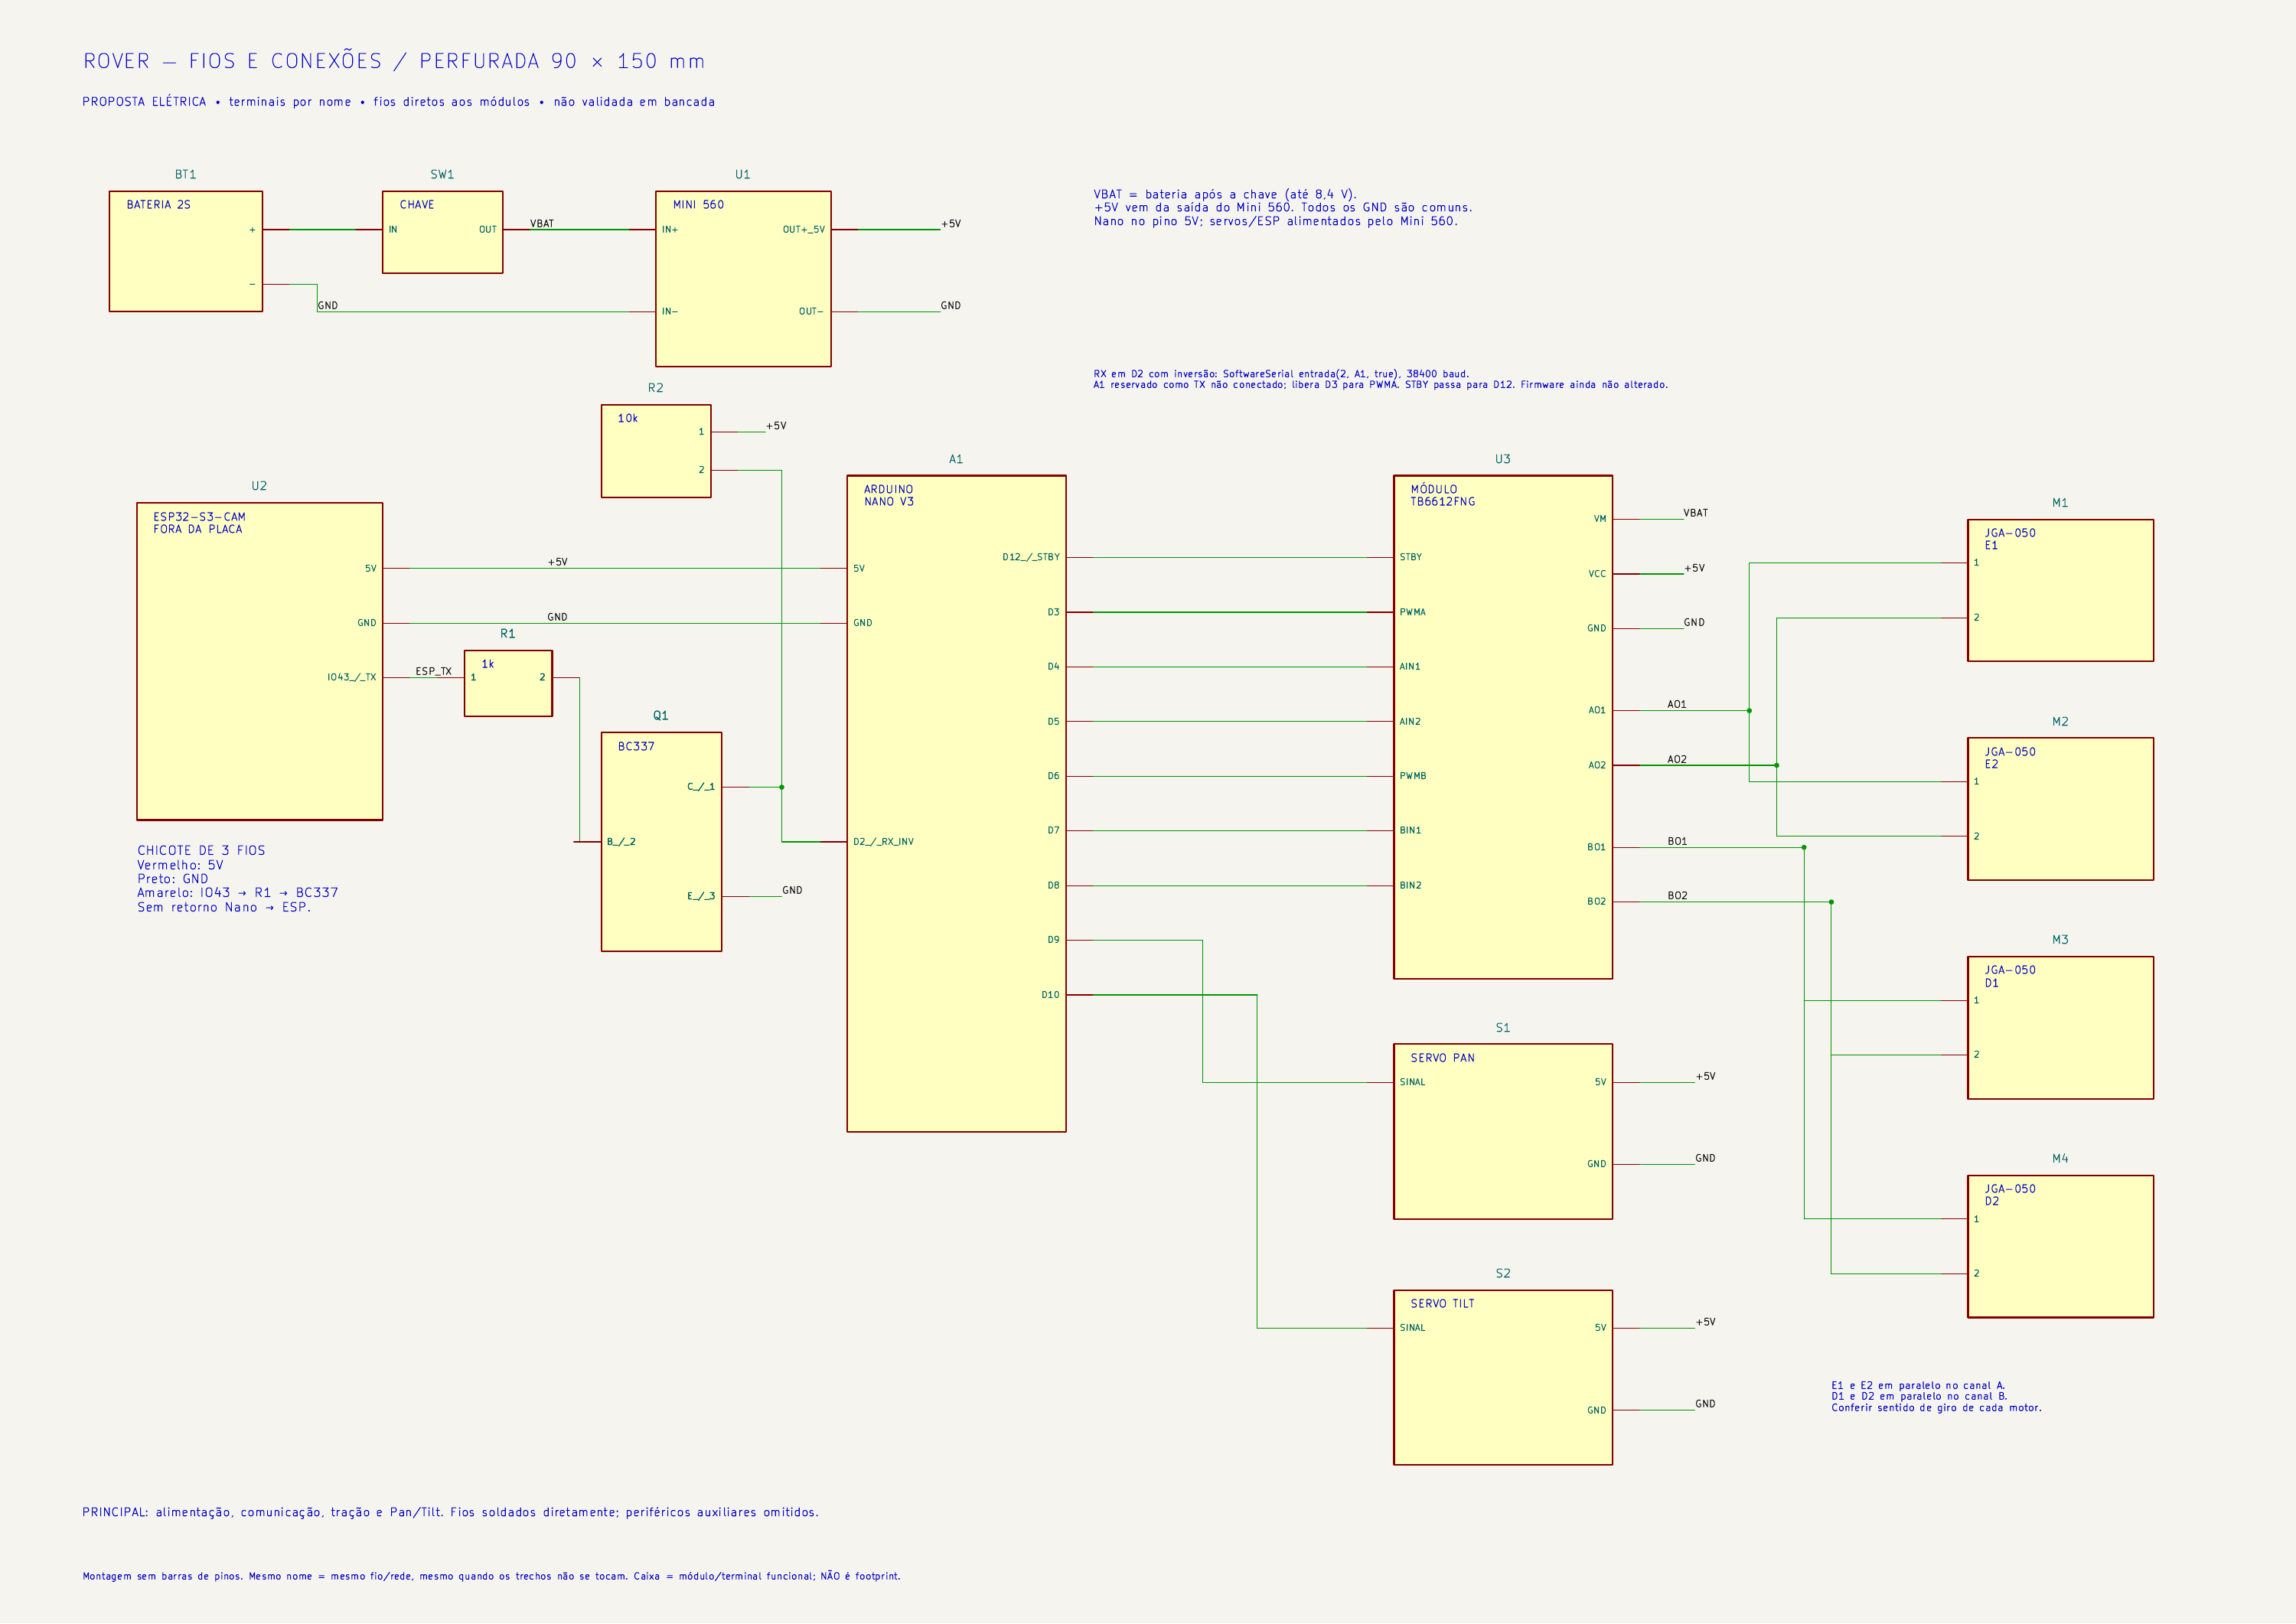
\includegraphics[width=0.92\textwidth]{kicad/rover_perfurada_90x150/rover_conexoes.png}
\caption{Esquema Elétrico Completo de Interligação (KiCad).}
\end{figure}

\vspace{0.3cm}

\begin{figure}[h!]
\centering
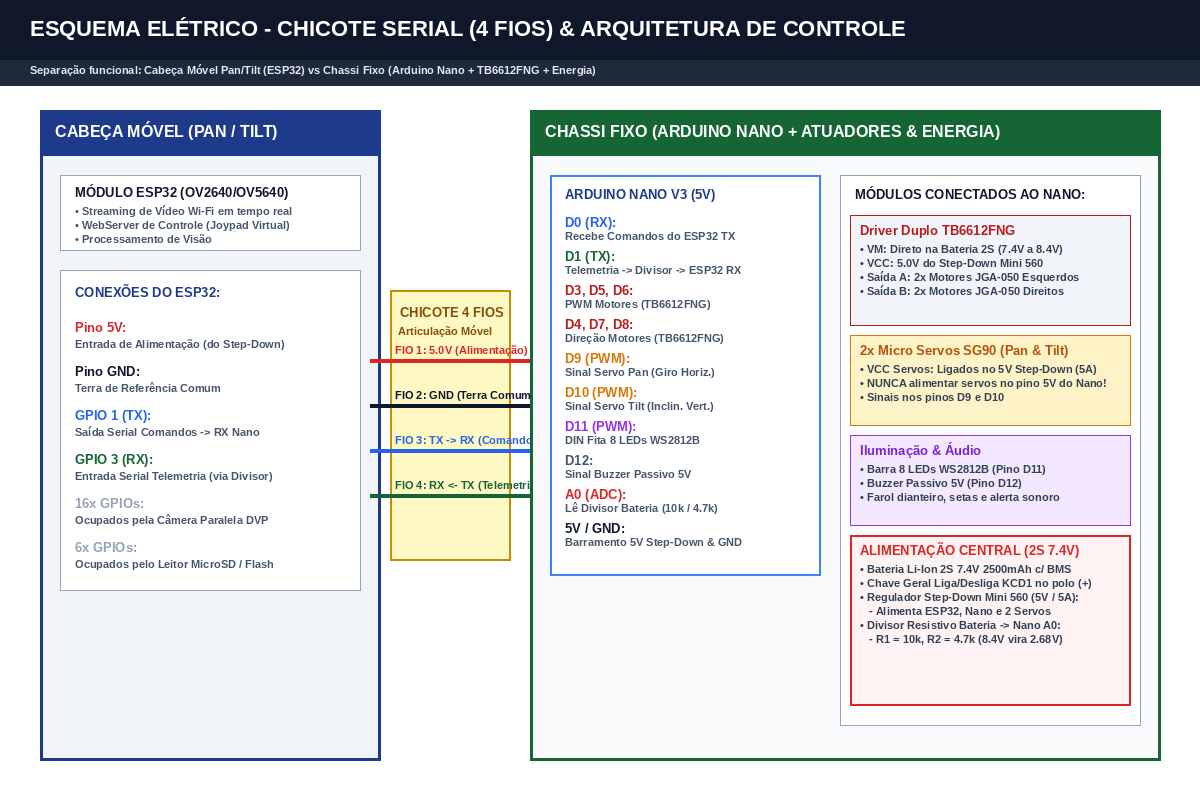
\includegraphics[width=0.8\textwidth]{esquema_eletrico_chicote_esp32_nano.png}
\caption{Arquitetura Distribuída: Cabeça Pan/Tilt (ESP32) vs Chassi Fixo (Nano).}
\end{figure}

\newpage

\section{Mapeamento Pino a Pino das Conexões}

\subsection{A. Distribuição de Alimentação e Terra}
\begin{table}[h!]
\centering
\small
\begin{tabularx}{\textwidth}{p{4.5cm} p{5.5cm} X}
\toprule
\rowcolor{tablehead} \color{white}\textbf{Ponto de Origem} & \color{white}\textbf{Ponto de Destino} & \color{white}\textbf{Descrição do Sinal} \\
\midrule
Bateria Li-Ion (+) & Entrada da Chave KCD1 & VBAT Bruto (7.4V nominal / 8.4V pico) \\
\rowcolor{tablezebra} Saída da Chave KCD1 & Step-Down Mini 560 (IN+) e TB6612 (VM) & VBAT Chaveado para alimentação e motores \\
Bateria Li-Ion (-) & Trilha Barramento GND & Referência 0V Geral \\
\rowcolor{tablezebra} Mini 560 (IN- e OUT-) & Trilha Barramento GND & GND de entrada e saída do regulador \\
Mini 560 (OUT+) & Trilha Barramento +5V & 5.0V estáveis (até 5A) para toda a lógica \\
\rowcolor{tablezebra} Trilha Barramento +5V & Nano (5V), TB6612 (VCC), ESP32 (5V), Servos (5V), R2 (10k) & Linha de alimentação lógica de 5V \\
Trilha Barramento GND & Nano (GND), TB6612 (GND), ESP32 (GND), Servos (GND), BC337 (E) & Linha de terra comum \\
\bottomrule
\end{tabularx}
\end{table}

\subsection{B. Comunicação Serial (Chicote ESP32 ➔ Inversor BC337 ➔ Nano)}
\begin{table}[h!]
\centering
\small
\begin{tabularx}{\textwidth}{p{4.5cm} p{5.5cm} X}
\toprule
\rowcolor{tablehead} \color{white}\textbf{Ponto de Origem} & \color{white}\textbf{Ponto de Destino} & \color{white}\textbf{Descrição do Sinal} \\
\midrule
ESP32 Pino 5V (Externo) & Trilha Barramento +5V & Fio 1 do chicote: Alimentação do ESP32 \\
\rowcolor{tablezebra} ESP32 Pino GND (Externo) & Trilha Barramento GND & Fio 2 do chicote: Terra de referência \\
ESP32 Pino IO43 TX (Externo) & Resistor R1 (1 k$\Omega$) & Fio 3 do chicote: Sinal serial de comandos (3.3V) \\
\rowcolor{tablezebra} Resistor R1 (1 k$\Omega$) & Transistor BC337 - Base (Pino 2) & Sinal para comutação do transistor \\
Transistor BC337 - Emissor (Pino 3) & Trilha Barramento GND & Referência de terra \\
\rowcolor{tablezebra} Transistor BC337 - Coletor (Pino 1) & Arduino Nano Pino D2 (RX) & Sinal convertido e invertido para 5V \\
Transistor BC337 - Coletor (Pino 1) & Resistor R2 (10 k$\Omega$) ao +5V & Pull-up de 5V para nível lógico HIGH \\
\bottomrule
\end{tabularx}
\end{table}

\subsection{C. Tração 4WD: Arduino Nano ➔ TB6612FNG ➔ Motores JGA16-050}
\begin{table}[h!]
\centering
\small
\begin{tabularx}{\textwidth}{p{4.5cm} p{5.5cm} X}
\toprule
\rowcolor{tablehead} \color{white}\textbf{Ponto de Origem} & \color{white}\textbf{Ponto de Destino} & \color{white}\textbf{Descrição do Sinal} \\
\midrule
Arduino Nano D12 & TB6612 Pino STBY & Habilitação da Ponte H (HIGH = Motores ativos) \\
\rowcolor{tablezebra} Arduino Nano D3 (PWM) & TB6612 Pino PWMA & Velocidade PWM dos Motores Esquerdos \\
Arduino Nano D4 & TB6612 Pino AIN1 & Direção 1 dos Motores Esquerdos \\
\rowcolor{tablezebra} Arduino Nano D5 & TB6612 Pino AIN2 & Direção 2 dos Motores Esquerdos \\
Arduino Nano D6 (PWM) & TB6612 Pino PWMB & Velocidade PWM dos Motores Direitos \\
\rowcolor{tablezebra} Arduino Nano D7 & TB6612 Pino BIN1 & Direção 1 dos Motores Direitos \\
Arduino Nano D8 & TB6612 Pino BIN2 & Direção 2 dos Motores Direitos \\
\rowcolor{tablezebra} TB6612 Saídas AO1 e AO2 & 2x Motores Esquerdos (Paralelo) & Alimentação dos motores esquerdos \\
TB6612 Saídas BO1 e BO2 & 2x Motores Direitos (Paralelo) & Alimentação dos motores direitos \\
\bottomrule
\end{tabularx}
\end{table}

\subsection{D. Servos da Câmera: Arduino Nano ➔ SG90}
\begin{table}[h!]
\centering
\small
\begin{tabularx}{\textwidth}{p{4.5cm} p{5.5cm} X}
\toprule
\rowcolor{tablehead} \color{white}\textbf{Ponto de Origem} & \color{white}\textbf{Ponto de Destino} & \color{white}\textbf{Descrição do Sinal} \\
\midrule
Arduino Nano D9 (PWM) & Header Servo Pan (Sinal Amarelo) & Sinal de controle Pan (Horizontal: 0° a 180°) \\
\rowcolor{tablezebra} Arduino Nano D10 (PWM) & Header Servo Tilt (Sinal Amarelo) & Sinal de controle Tilt (Vertical: 0° a 180°) \\
Trilha Barramento +5V & Headers dos Servos (Pino Vermelho) & Alimentação dedicada via Mini 560 \\
\rowcolor{tablezebra} Trilha Barramento GND & Headers dos Servos (Pino Marrom) & Referência de terra \\
\bottomrule
\end{tabularx}
\end{table}

\newpage

\section{Dicas Práticas de Soldagem e Layout}

\begin{itemize}[leftmargin=1.5em, itemsep=0.5em]
    \item \textbf{Barras de Pinos Fêmea (Soquetes):} Não solde o Arduino Nano nem o TB6612 diretamente na perfurada. Solde soquetes fêmea de 2.54 mm para encaixar as placas. Isso previne danos térmicos e facilita substituições ou reprogramações fora do robô.
    \item \textbf{Trilhas Mestras de Alimentação:} Em placas de ilhas isoladas, solde duas linhas de fio rígido estanhado contínuo atravessando a placa (uma para GND e outra para +5V), facilitando conectar qualquer componente à ilha vizinha.
    \item \textbf{Headers Macho para Cabos Externos:} Use headers macho de 3 pinos para os servos (\texttt{[SINAL | 5V | GND]}) e para o chicote do ESP32 (\texttt{[5V | GND | TX]}), dispensando cortes nos cabos originais.
    \item \textbf{Fios de Potência Curtos:} Mantenha os condutores do Step-Down e saídas dos motores curtos e com bitola adequada (AWG 22 a 24).
\end{itemize}

\vspace{0.5cm}

\begin{figure}[h!]
\centering
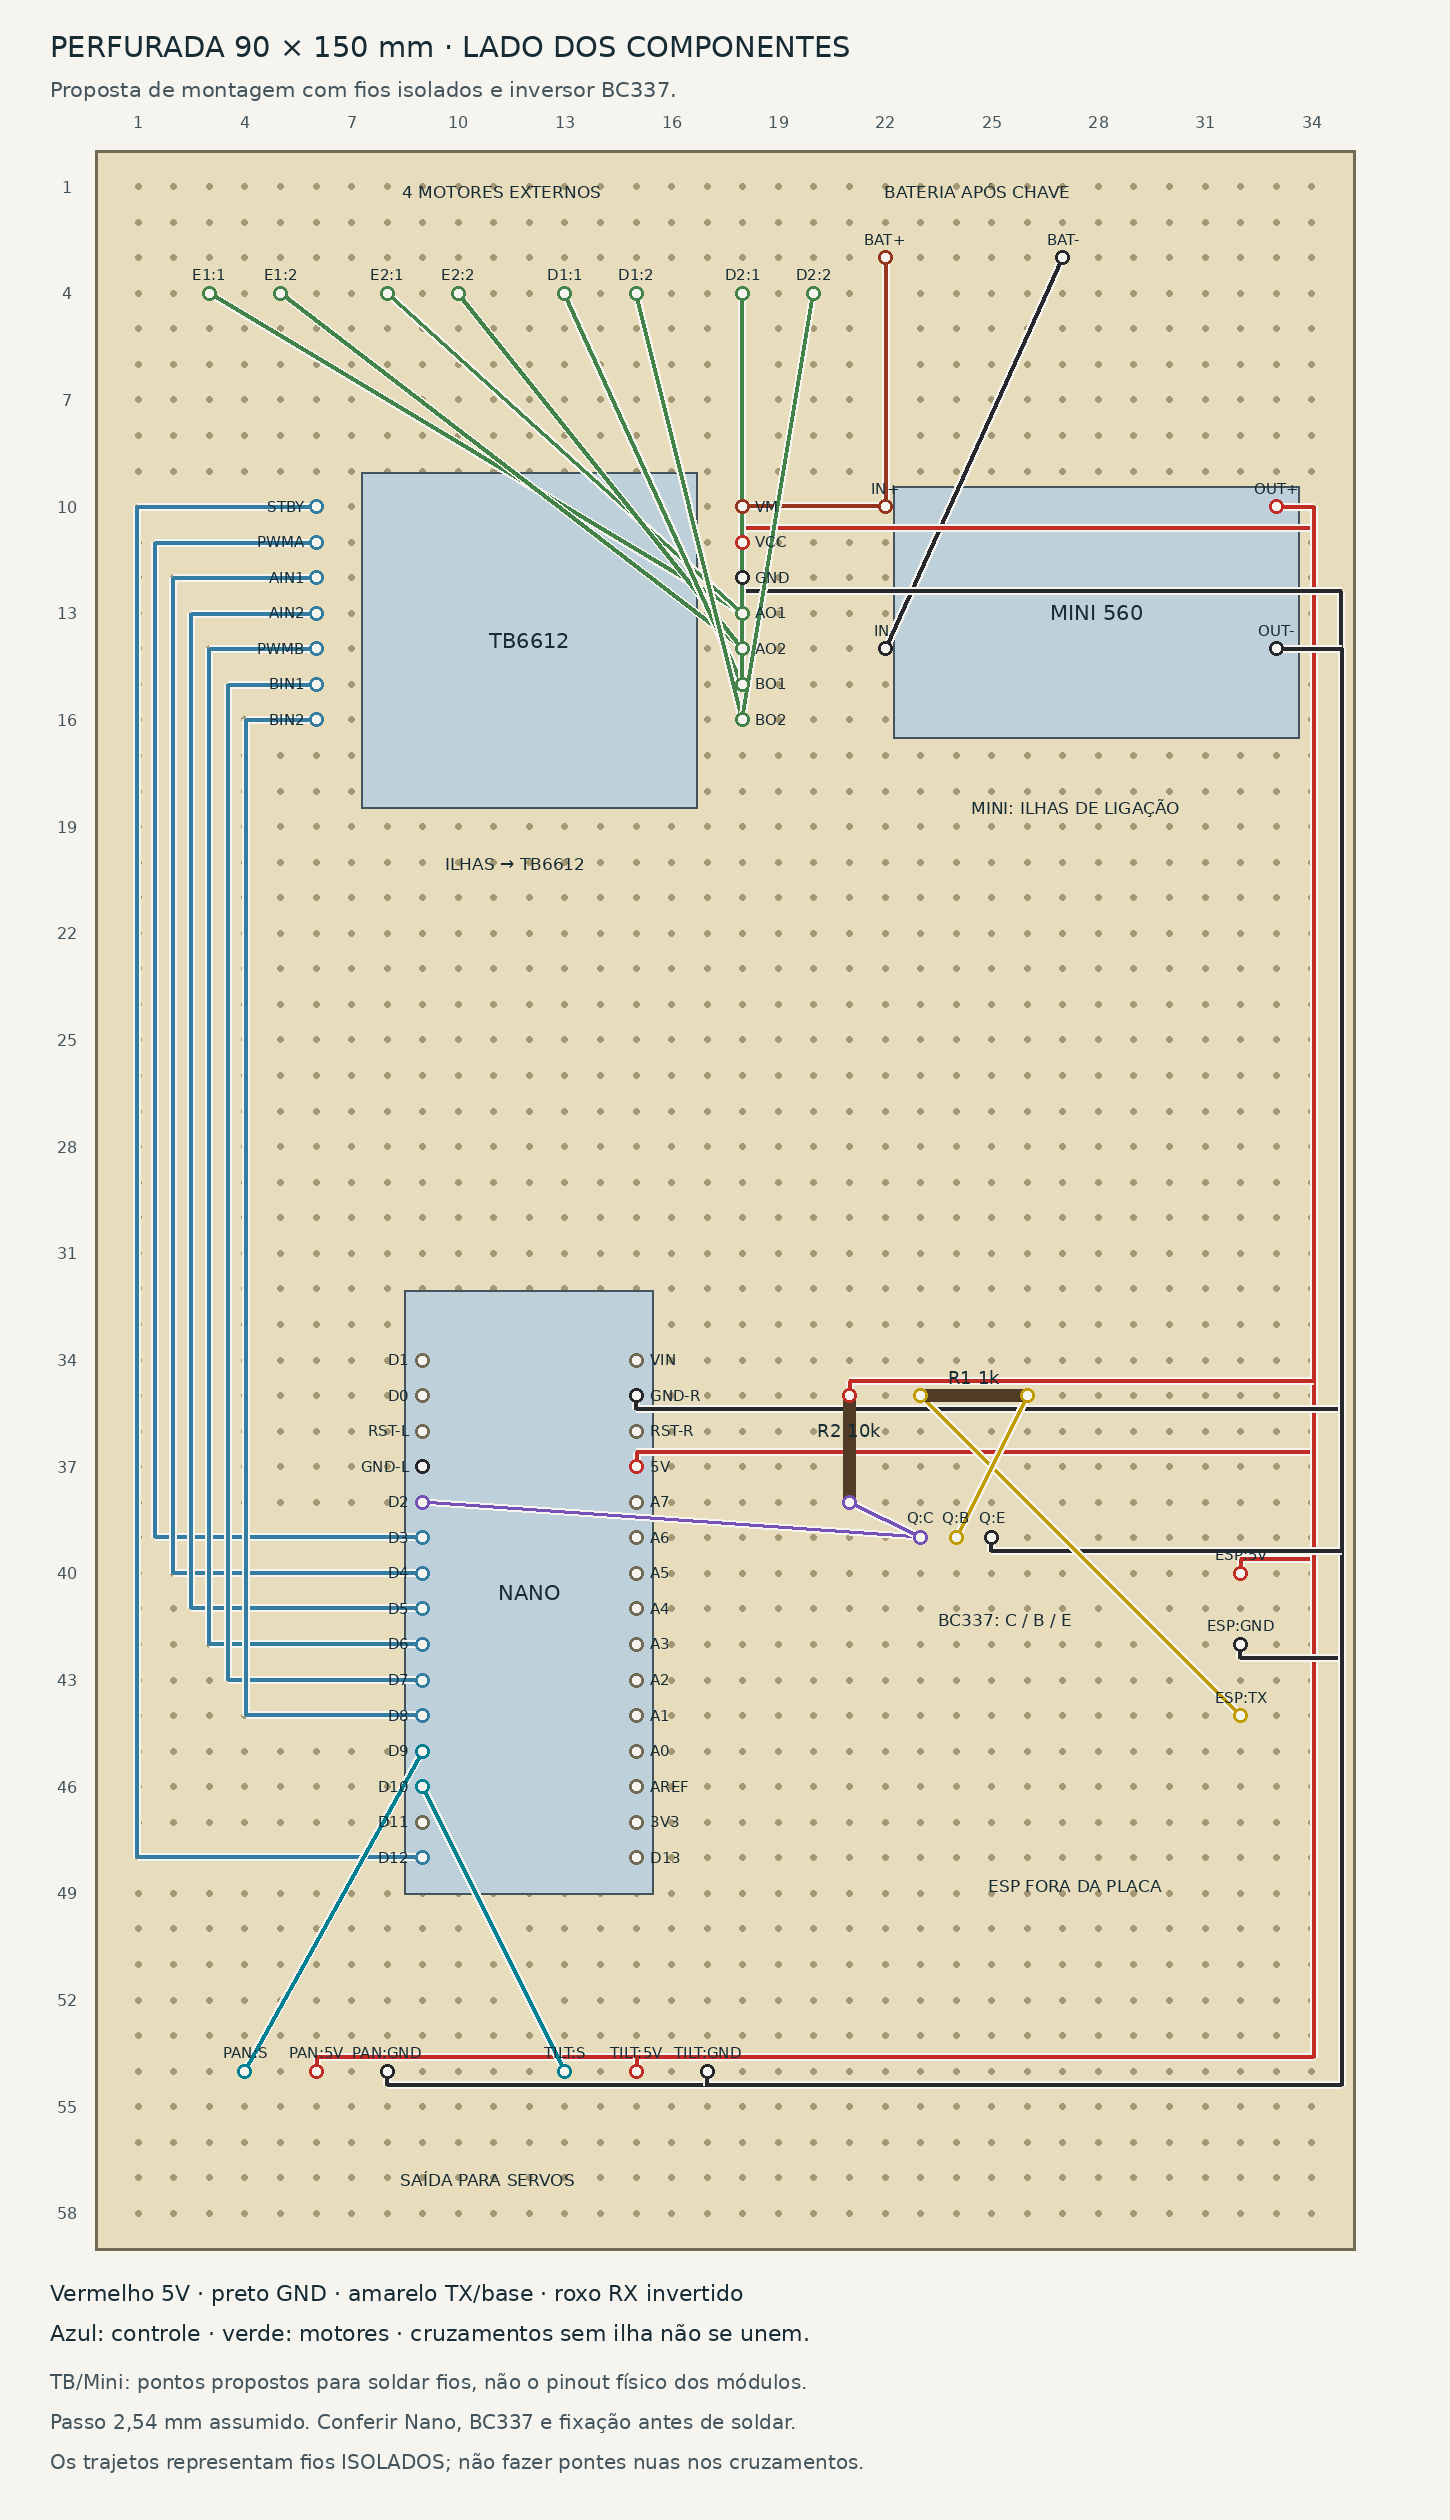
\includegraphics[width=0.58\textwidth]{kicad/rover_perfurada_90x150/montagem_superior.png}
\caption{Sugestão de Layout Físico na Placa Perfurada (90 x 150 mm).}
\end{figure}

\end{document}
